\documentclass[lettersize,preprint]{elsarticle}
\usepackage{amsmath,amsfonts}
\usepackage{subfig}
\usepackage{url}
\usepackage{graphicx}
\usepackage{siunitx}

\usepackage{multirow}

\usepackage{tikz}
\usepackage{makecell}

\usepackage{csquotes}
\usepackage{wrapfig}
\usepackage{parskip}
\usepackage[acronym]{glossaries}
\makeglossaries

\usetikzlibrary{fadings, fit, backgrounds, calc,arrows, arrows.meta,decorations.markings,spy}


\tikzset{
    cross/.pic = {
    \draw[rotate = 45] (-#1,0) -- (#1,0);
    \draw[rotate = 45] (0,-#1) -- (0, #1);
    }
}


\tikzset{
  camera/.pic = {
    \fill [] (-0.5,-0.5) rectangle (0.5,0.5);
    \draw [] (0.0,0.0) 
    -- (-0.6,1.3) 
    -- (0.6,1.3) 
    -- cycle;
  }
}
\tikzset{
  camera_right/.pic = {
    \fill [red] (-0.5,-0.5) rectangle (0.5,0.5);
    \draw [red] (0.0,0.0) 
    -- (-0.6,1.3) 
    -- (0.6,1.3) 
    -- cycle;
  }
}


\tikzset{
  uav_frame/.pic = {
    \draw [line width=0.6mm] (-1,-1) -- (1,1);
    \draw [line width=0.6mm] (-1,1) -- (1,-1);
    \fill [black] (-0.4,-0.4) rectangle (0.4,0.4);
  }
}

\tikzset{
  observer/.pic = {
    \pic at (0,0) {uav_frame};
    \pic [rotate=70, scale=0.35] at (-0.3,0.35) {camera};
    \pic [rotate=-70, scale=0.35] at (0.4,0.35) {camera_right};
  }
}

\tikzset{
  tx/.pic = {
    \pic at (0,0) {uav_frame};
    \filldraw [red] (-1,-1) circle (3pt);
    \filldraw [red] (-1,1) circle (3pt);
    \filldraw [red] (1,-1) circle (3pt);
    \filldraw [red] (1,1) circle (3pt);
  }
}




\makeatletter
\let\AC@footnote\@gobble
\makeatother


\newcommand{\B}{$\mathcal{B}$}
\newcommand{\BS}{$\mathcal{B}^*$}
\newcommand{\D}{$\mathcal{D}$}
\newcommand{\ps}{\emph{p-state}}
\newcommand{\ts}{\emph{t-series}}

\newacronym{AMT}{AMT}{Active blinking Marker Tracking}
\newacronym{IR}{IR}{Infrared}
\newacronym{GNSS}{GNSS}{Global Navigation Satellite System}
\newacronym{MOCAP}{mo-cap}{Motion capture}
\newacronym{MRS}{MRS}{Multi-robot Systems Group}
\newacronym{MAV}{MAV}{Micro-scale Unmanned Aerial Vehicle}
\newacronym{UWB}{UWB}{Ultra-wideband}
\newacronym{GPU}{GPU}{Graphics Processing Unit}
\newacronym{VIO}{VIO}{Visual Inertial Odometry}
\newacronym{UAV}{UAV}{Unmanned Aerial Vehicle}
\newacronym{UGV}{UGV}{Unmanned Ground Vehicle}
\newacronym{UVDAR}{UVDAR}{UltraViolet Direction And Ranging}
\newacronym{RTK}{RTK}{Real-Time Kinematic}
\newacronym{SIFT}{SIFT}{Scale-invariant Feature Transform}
\newacronym{wrt}{w.r.t.}{With Respect To}
\newacronym{4DHT}{4DHT}{4D Hough Transform}
\newacronym{UV}{UV}{Ultraviolet}
\newacronym{TX}{TX}{Transmitter}
\newacronym{RX}{RX}{Receiver}
\newacronym{FOV}{FOV}{Field of View}
\newacronym{LED}{LED}{Light-Emitting Diode}
\newacronym{RF}{RF}{Radio Frequency}
\newacronym{OCC}{OCC}{Optical Camera Communication}
\newacronym{DVS}{DVS}{Dynamic Vision System}
\newacronym{CMOS}{CMOS}{Complementary Metal-Oxide-Semiconductor}
\newacronym{LoS}{LoS}{Line of Sight}
\newacronym{OOK}{OOK}{On-Off Keying}
\newacronym{CNN}{CNN}{Convolutional Neural Network}
\newacronym{GM-PHD}{GM-PHD}{Gaussian Mixture Probability Hypothesis Density}
\newacronym{RSS}{RSS}{Resident Set Size}
\newacronym{FAST}{FAST}{Features from Accelerated Segment Test}
 
\journal{Robotics and Autonomous Systems}

\begin{document}

\begin{frontmatter}

\title{Towards Agile Swarming in Real World: Onboard Relative Localization with Fast Tracking of Active Blinking Markers\tnoteref{t1}}
\tnotetext[t1]{This work was funded by CTU grant no SGS23/177/OHK3/3T/13, by the Czech Science Foundation (GAČR) under research project no. 23-07517S and by the European Union under the project Robotics and advanced industrial production (reg. no. CZ.02.01.01/00/22\_008/0004590).}

\author[1]{Tim Lakemann\corref{cor1}}
\ead{lakemtim@fel.cvut.cz}
\author[1,2]{Daniel Bonilla Licea}
\author[1]{Viktor Walter}
\author[1]{Tomáš Báča}
\author[1]{Martin Saska}


\cortext[cor1]{Corresponding author, +420-22435-7255}
\affiliation[1]{organization={Czech Technical University},%Department and Organization
            addressline={Karlovo namesti 13}, 
            city={Prague},
            postcode={121 35}, 
            country={Czech Republic}}
\affiliation[2]{organization={Mohammed VI Polytechnic University}, 
country={Morocco}}

\begin{abstract}
A novel onboard tracking approach enabling vision-based relative localization and communication using \gls{AMT} is introduced in this article.
Active blinking markers on multi-robot team members improve the robustness of relative localization for aerial vehicles in tightly coupled swarms during real-world deployments, while also serving as a resilient communication channel.
Traditional tracking algorithms struggle to track fast moving blinking markers due to their intermittent appearance in the camera frames.
\gls{AMT} addresses this by using weighted polynomial regression to predict the future appearance of active blinking markers while accounting for uncertainty in the prediction.
In outdoor experiments, the \gls{AMT} approach outperformed state-of-the-art methods in tracking density, accuracy, and complexity. 
The experimental validation of this novel tracking approach for relative localization involved testing motion patterns motivated by our research on agile multi-robot deployment.
\end{abstract}

% \begin{highlights}
%   \item novel method for tracking blinking markers in agile flight
%   \item Uncertainty estimates from weighted regression define a search window for accuracy
%   \item A recovery mechanism re-tracks markers after failures, increasing reliability
%   \item It is an enabling technology for fast, vision-only relative localization.
% \end{highlights}

\begin{keyword}
Visual Tracking, Localization, Multi-Robot Systems, Computer Vision for Automation
\end{keyword}

\end{frontmatter}

\section{Introduction}
In various applications, collaborative multi-\gls{UAV} systems enhance redundancy and improve efficiency compared to single-robot systems~\cite{chungSurveyAerialSwarm2018}.
Accurate localization of team members is crucial for collision avoidance and effective collaborative task execution \cite{chungSurveyAerialSwarm2018,chenSurveyRobotSwarms2022}.
\gls{GNSS} alone is insufficient for close formation flight in such environments due to its meter-level accuracy, limited availability (e.g., indoors, underground), and vulnerability to jamming and spoofing \cite{xuDecentralizedVisualInertialUWBFusion2020a, gaoVIDORobustConsistent2023}.
While \gls{RTK}-\gls{GNSS} and motion capture systems offer centimeter-level accuracy, they rely on external infrastructure or public networks, limiting their practicality in many real-world environments \cite{chungSurveyAerialSwarm2018,chenSurveyRobotSwarms2022, wuRealizationRemoteMonitoring2022}.
Alternatively, onboard \gls{UWB} provides comparable precision in distance estimation without requiring external infrastructure.
However, its effectiveness can be limited by radio jamming, interference, and channel saturation, and for pose measurements, a \gls{UWB} network with external anchors is required \cite{xuDecentralizedVisualInertialUWBFusion2020a,jiangIndoorOutdoorSeamless2021, queraltaUWBbasedSystemUAV2020, zhouSwarmMicroFlying2022}.
Camera-based mutual relative localization offers a robust and cost-efficient solution for multi-robot systems without external infrastructure \cite{schillingVisionBasedDroneFlocking2021}. 
This method of relative localization relies on camera-based object detection and tracking algorithms.
In recent works \cite{xuDecentralizedVisualInertialUWBFusion2020a,schillingVisionBasedDroneFlocking2021, ohMarkerBasedLocalizationSystem2023}, such algorithms often use \glspl{CNN}, which are computationally intensive, have low output rates on general purpose PCs, are highly dependent on illumination, and are typically limited to the specific robot platforms included in the training dataset.
Passive markers attached to robot platforms for visual localization are cost-effective and easy to deploy in multi-robot systems \cite{romero-ramirezSpeededDetectionSquared2018a,krajnikExternalLocalizationSystem2013}. 
However, they are also dependent on illumination and require planar surfaces for attachment, which is impractical for small robots.
To overcome these limitations, active markers in the form of \glspl{LED} can be attached to team members, allowing for efficient background separation and reliable operation in challenging outdoor/indoor environments \cite{stuckeyRealTimeOpticalLocalization2024,whiteOpticalSpatialLocalization2019, teixeiraVIRPEVisualInertialRelative2018, walterUVDARSystemVisual2019, faesslerMonocularPoseEstimation2014, limHemisphericalInfraRedIR2022}.
When using constant power, the markers are visible in consecutive camera frames, allowing for the use of classical tracking algorithms, such as the Kalman filter \cite{jinVisionTrackingSystem2016b, doVisibleLightCommunicationBased2019, huangImprovedTargetSignal2018}. 
This reduces team member differentiation and increases the risk of false detections from outdoor sunlight, reflections, and indoor artificial lighting.

\begin{figure}[t]
  \centering
  \scalebox{1.5}{\begin{tikzpicture}[spy using outlines={size=12mm}, rectangle, connect spies]
  \node[anchor=south west,inner sep=0] (a) at (0,0) { 
  \includegraphics[width=0.45\textwidth]{desert.png}};

  \spy[width=1.45cm, height=2.5cm, magnification=3, 
    fill=none, 
    line width=1.pt,
    color=red,
    connect spies, 
     spy connection path={\draw[thick](tikzspyonnode) -- (tikzspyinnode);}]
    on (2.9, .6) in node[opacity=1, thick] at (7., 1.3);

\end{tikzpicture}}
  \caption{Six agile swarm members flying in challenging desert conditions, relying on \glsentryshort{UVDAR}-based relative localization as used in this work.}
  \vspace{-5pt}
  \label{fig:intro:overview}
\end{figure}

These challenges may be overcome by modulating the blinking frequencies of the markers.
By using, e.g. \gls{OOK}, the team members can share information and uniquely identify each other \cite{whiteOpticalSpatialLocalization2019,whiteRobustOpticalSpatial2019,diasOnboardVisionbased3D2016, stuckeyOpticalSpatialLocalization2021,stuckeySpatialLocalizationAttitude2022}.
Conventional tracking algorithms are inadequate for tracking active blinking markers due to their intermittent appearance and movement in the camera image of the \gls{RX}, which is caused by relative motion between team members \cite{chenUltravioletBasedUAVSwarm2022}.
Additionally, recent studies on agile multi-robot teams have shown maximum trajectory speeds of \SI{2}{\meter\per\second} in object-dense outdoor environments \cite{zhouSwarmMicroFlying2022}, and \SI{7.4}{\meter\per\second} in object-sparse indoor environments using external infrastructure, such as a motion capture system \cite{ryouCooperativeMultiAgentTrajectory2022}.
Even at lower inter-agent speeds, effective tracking algorithms are crucial for relative localization, as relative motion within these teams surpasses the abilities of current state-of-the-art methods.

We propose the novel \glsfirst{AMT} approach, a system-agnostic method for tracking light sources attached to multi-robot team members.
By using motion models and the constraints of cooperating aerial robots, the \gls{AMT} approach solves the tracking problem by fusing the past motion of blinking light sources to estimate the next expected location of the team members in the image.
This proposed approach enables vision-based relative localization of blinking light sources attached to fast moving \glspl{UAV} (Fig. \ref{fig:intro:overview}).
The source code\footnote{\url{https://github.com/TimLakemann/ami.git}} and a demonstration video\footnote{\url{https://mrs.fel.cvut.cz/towards-agile-swarming-in-real-world}} can be found online.


\section{State of the Art and Contribution}\label{sec:sota}

Active blinking markers attached to the \gls{UAV} frame enhance reliability and enable unique identification, while also reducing the computational cost of object detection algorithms.
In \cite{whiteOpticalSpatialLocalization2019}, White \emph{et al.} tracked a static \gls{LED} ring using spatial-temporal difference images, with the ring blinking at half the frame rate of the camera. 
This work was extended in~\cite{whiteRobustOpticalSpatial2019} by attaching the \gls{LED} ring to a \gls{UAV} and tracked it with a stationary camera.
However, using difference images restricts the blinking frequency for all team members to half the frame rate of the camera, making it difficult to distinguish between the transmitting \glspl{UAV} (\glsentryshortpl{TX}).

Breitenmoser \emph{et al.} developed a mutual relative localization system using active and passive markers in \cite{breitenmoserMonocularVisionbasedSystem2011}, achieving centimeter-level accuracy in indoor experiments. 
However, they observed that different marker frequencies could enhance robustness in differentiating robot targets. 
Additionally, the system was not tested for cross-talk detection when robots were close.

In \cite{stuckeyOpticalSpatialLocalization2021, stuckeySpatialLocalizationAttitude2022,censiLowlatencyLocalizationActive2013,ebmerRealtime6DoFPose2024}, the authors tracked a \gls{UAV} with blinking markers using a \gls{DVS}, which requires different tracking approaches compared to \gls{CMOS} cameras.
Cenci \emph{et al.} extracted the individual frequencies associated with \gls{IR}-markers attached to a \gls{UAV} in an indoor environment \cite{censiLowlatencyLocalizationActive2013}.
In \cite{ebmerRealtime6DoFPose2024}, a \gls{DVS} was used to track a marker board with four blinking \glspl{LED}. 
They tested the system in indoor and outdoor environments with a working distance of up to 10 meters.
However, their system fails to address occlusions or situations where the \glspl{LED} appear close together in the image. Further, \glspl{DVS} typically have a limited \gls{FOV} and are more expensive than \gls{CMOS} cameras \cite{walterFastMutualRelative2018a}. 
To our knowledge, systems using \glspl{DVS} do not handle tracking when both the \gls{RX} and \glsentryshort{TX} are moving, making them impractical for mutual relative localization and, consequently, for multi-robot systems.

In \cite{gorseOpticalCameraCommunication2018}, the authors changed the light intensity of \gls{IR}-\glspl{LED} to represent the two different bit states.
Changes in light intensity are effective in indoor environments.
However, it causes ambiguities in outdoor environments due to higher background brightness and noise caused by sunlight.

In \cite{diasOnboardVisionbased3D2016}, the authors used a combination of three blue non-blinking markers for relative localization and one red blinking marker for identification attached to the frame of a \gls{UAV} for indoor relative localization.
This combination enables continuous tracking by the non-blinking markers and unique identification by the blinking markers.
However, non-blinking markers reduce transmission bandwidth and reliability. At the same time, reliance on the visible spectrum increases dependence on lighting conditions and limits the operational range of \glspl{UAV} in outdoor environments.


\subsection{The UVDAR system}\label{sec:uvdar}
The \glsfirst{UVDAR} system provides relative localization and communication for \glspl{UAV} operating in both indoor and outdoor environments \cite{walterUVDARSystemVisual2019, walterFastMutualRelative2018a, walterMutualLocalizationUAVs2018, petracekBioinspiredCompactSwarms2021,horynaUVDARCOMUVBasedRelative2022}.
s in varying lighting conditions \cite{walterFastMutualRelative2018a}.
The system uses \gls{UV}-\glspl{LED} on the arms of a target \gls{UAV} for data transmission in combination with calibrated grayscale cameras with \gls{UV} band-pass filters (Fig. \ref{fig:uav_platform}) attached on observer \glspl{UAV} \cite{liceaOpticalCommunicationbasedIdentification2023}.
The band-pass filters remove the most visible light, making the blinking markers appear as bright white spots in the camera image of the observer.
These are then processed using a \gls{FAST}-like procedure and non-maxima suppression to extract the center pixel of each marker \cite{walterFastMutualRelative2018a,walterMutualLocalizationUAVs2018}. 

\begin{figure}[t]
  \centering
    \includegraphics[width=0.6\textwidth]{UVDARsystem.pdf}
      \caption{\gls{UAV} equipped with the UVDAR system \cite{liceaOpticalCommunicationbasedIdentification2023}. }
      \vspace{-5pt}
      \label{fig:uav_platform}%
\end{figure}

Multiple \gls{UV}-\glspl{LED} on a single multirotor's arm emit an identical sequence, recognized as a blinking marker (green box in Fig. \ref{fig:uav_platform}).
These binary sequences are stored in a dictionary \D{} that contains \gls{LED}-IDs associated with each sequence \cite{liceaOpticalCommunicationbasedIdentification2023}.
In our previous work \cite{walterMutualLocalizationUAVs2018}, we solved the tracking problem of the blinking markers by using the Hough Transform for 3D line extraction.
The search for maxima in the Hough Space introduces high computational load and memory usage. 
Additionally, the line approximation of the movement of the marker in the image is insufficient for fast and agile maneuvers of the multi-robot system.

\subsection{Contribution}\label{subsec:contribution}
This work is motivated by the need for reliable mutual visual tracking in agile multi-robot systems operating in real-world (outdoor/indoor) environments, particularly in tightly cooperating swarms.
The proposed approach was integrated with the \gls{UVDAR} system \cite{walterFastMutualRelative2018a}, but it can also be applied to any multi-robot framework using active blinking markers.
We validated its effectiveness through outdoor experiments, demonstrating substantial performance improvements over the state-of-the-art method.
The main contributions of this work are the following:
\begin{enumerate}
  \item We propose a novel approach for tracking blinking markers across consecutive images, considering the requirements of onboard mutual relative localization under the constraints of agile flight.
    \item We use uncertainty estimates from weighted polynomial regression to define a search window for future marker appearances, enhancing tracking accuracy under dynamic conditions.
    \item We propose a recovery mechanism that re-tracks blinking markers after tracking failures, significantly increasing reliability for the real-world deployment of closely cooperating teams.
    \item We provide an enabling technology for fast, agile aerial multi-robot systems with vision-only relative localization.
\end{enumerate}


\section{\glsentryfull{AMT}}\label{sec:ami}

The proposed \gls{AMT} approach enables the tracking of multiple moving blinking light sources across consecutive image captures, allowing the extraction of individual blinking sequences, which is essential for agile multi-\gls{UAV} systems.
Positions of extracted bright points (see Sec. \ref{sec:uvdar}) from a recent camera image are stored in the set $\mathcal{P}_t = \{p_{t,1},\hdots, p_{t,k}, \hdots,p_{t,m}\}$, where $t$ is the timestamp of the image acquisition.
These positions are referred to as \emph{image-points}.

The \gls{AMT} approach requires knowledge of the maximum number of consecutive zeros ($b_{m,0}$) of the sequences emitted by the blinking markers; this is necessary to keep only valid entries in the dynamic buffer, named \B{}.
The buffer \B{} tracks potential matches between the \emph{image-points} and sequences emitted by the blinking markers of the \glsentryshortpl{TX} and stores the associations in \ts{}.
An \emph{image-point} is converted to a point state (\emph{p-state}) as soon as it is inserted into \B{}. 
A \ps{} contains the image capture time, pixel coordinates, and \emph{state}, which can be either `1' (marker \enquote{on}) or `0' (marker \enquote{off}).
\begin{figure}
  \centering
  \vspace{-8pt}
  \scalebox{0.5}{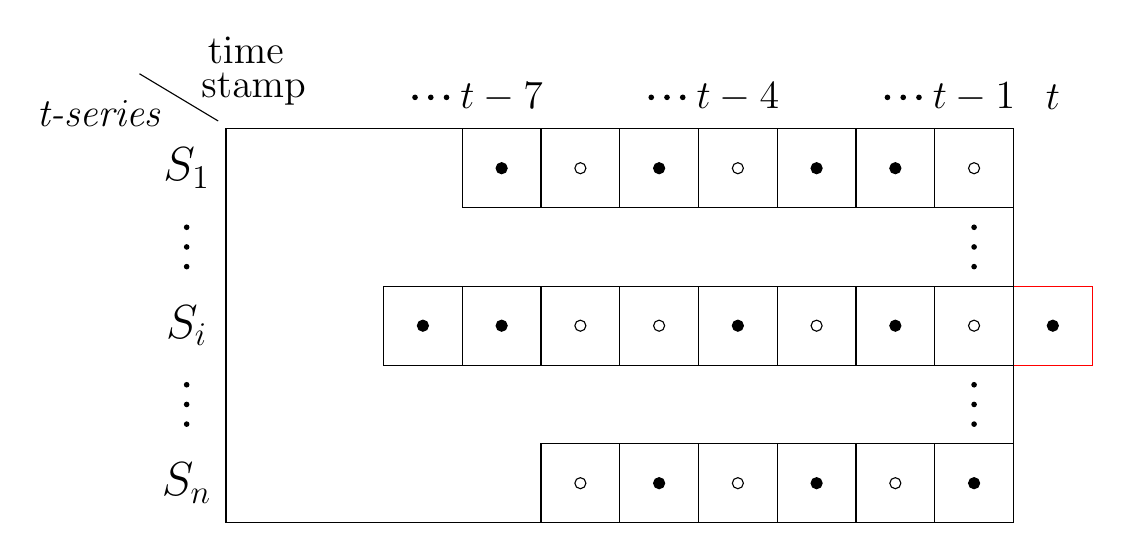
\begin{tikzpicture}

    \draw (3,13) rectangle ++(1,1);
    \draw (4,13) rectangle ++(1,1);
    \draw (5,13) rectangle ++(1,1);
    \draw (6,13) rectangle ++(1,1);
    \draw (7,13) rectangle ++(1,1);
    \draw (8,13) rectangle ++(1,1);
    \draw (9,13) rectangle ++(1,1);

    \draw (2,11) rectangle ++(1,1);
    \draw (3,11) rectangle ++(1,1);
    \draw (4,11) rectangle ++(1,1);
    \draw (5,11) rectangle ++(1,1);
    \draw (6,11) rectangle ++(1,1);
    \draw (7,11) rectangle ++(1,1);
    \draw (8,11) rectangle ++(1,1);
    \draw (9,11) rectangle ++(1,1);


    \filldraw (9.5,12.75) circle (0.8pt);
    \filldraw (9.5,12.5) circle (0.8pt);
    \filldraw (9.5,12.25) circle (0.8pt);

    \filldraw (9.5,10.75) circle (0.8pt);
    \filldraw (9.5,10.5) circle (0.8pt);
    \filldraw (9.5,10.25) circle (0.8pt);

    \draw (4,9) rectangle ++(1,1);
    \draw (5,9) rectangle ++(1,1);
    \draw (6,9) rectangle ++(1,1);
    \draw (7,9) rectangle ++(1,1);
    \draw (8,9) rectangle ++(1,1);
    \draw (9,9) rectangle ++(1,1);

    \filldraw[black] (2.5,11.5) circle (2pt);
    \filldraw[black] (3.5,11.5) circle (2pt);
    \draw[black][black] (4.5,11.5) circle (2pt);
    \draw[black] (5.5,11.5) circle (2pt);
    \filldraw[black] (6.5,11.5) circle (2pt);
    \draw[black] (7.5,11.5) circle (2pt);
    \filldraw[black] (8.5,11.5) circle (2pt);
    \draw[black] (9.5,11.5) circle (2pt);

    \filldraw[black] (3.5,13.5) circle (2pt);
    \draw[black] (4.5,13.5) circle (2pt);
    \filldraw[black] (5.5,13.5) circle (2pt);
    \draw[black] (6.5,13.5) circle (2pt);
    \filldraw[black] (7.5,13.5) circle (2pt);
    \filldraw[black] (8.5,13.5) circle (2pt);
    \draw[black] (9.5,13.5) circle (2pt);

    \draw[black] (4.5,9.5) circle (2pt);
    \filldraw[black] (5.5,9.5) circle (2pt);
    \draw[black] (6.5,9.5) circle (2pt);
    \filldraw[black] (7.5,9.5) circle (2pt);
    \draw[black] (8.5,9.5) circle (2pt);
    \filldraw[black] (9.5,9.5) circle (2pt);

    \node at (0.25, 15.) [align=left] {\Large time};
    \node at (0.35, 14.5) [align=left] {\Large stamp};
    
    \node at (-1.6,14.2) [align=left] {\Large \ts{}};
    \draw (-.1,14.1) -- (-1.1,14.7);


    \node at (-0.5,13.5) {\LARGE$S_{1}$};

    \node at (9.5,14.4) {\Large{$t-1$}};
    \node at (6.5,14.4) {\Large{$t-4$}};

    \node at (3.5,14.4) {\Large{$t-7$}};
    \node at (10.5,14.4) {\Large{$t$}};

    \filldraw (8.8,14.4) circle (0.8pt);
    \filldraw (8.6,14.4) circle (0.8pt);
    \filldraw (8.4,14.4) circle (0.8pt);
    
    \filldraw (5.8,14.4) circle (0.8pt);
    \filldraw (5.6,14.4) circle (0.8pt);
    \filldraw (5.4,14.4) circle (0.8pt);

    \filldraw (2.8,14.4) circle (0.8pt);
    \filldraw (2.6,14.4) circle (0.8pt);
    \filldraw (2.4,14.4) circle (0.8pt);
    \filldraw (-0.5,12.75) circle (0.8pt);
    \filldraw (-0.5,12.5) circle (0.8pt);
    \filldraw (-0.5,12.25) circle (0.8pt);

    \filldraw (-0.5,10.75) circle (0.8pt);
    \filldraw (-0.5,10.5) circle (0.8pt);
    \filldraw (-0.5,10.25) circle (0.8pt);

    \filldraw[black] (10.5,11.5) circle (2pt);
    \draw [red] (10,11) rectangle ++(1,1);
    \node at (-0.5,11.5) {\LARGE$S_{i}$};
    \node at (-0.5,9.5) {\LARGE$S_{n}$};
    \draw (0,9) rectangle ++(10,5);


\end{tikzpicture}
}
    \caption{\B{} contains multiple \ts{} ($S_1$, $\hdots,S_{n}$), each with multiple \emph{p-states}. Black circles indicate \enquote{on}-state; white circles indicate \enquote{off}-state of blinking marker. Red rectangle: new \ps{} inserted into $S_i$.}
  \label{figamtbuffer}
\end{figure}
Fig. \ref{figamtbuffer} provides an overview of \B{} and Sec. \ref{subsecamtbuffer} further explains the concept of \B{} and \ts{}.
The \gls{AMT} approach is divided into three parts:
\begin{enumerate}
  \item \emph{Local Search} (Sec. \ref{subsecamtlocal_search}): uses the markers' expected maximal speed in the image to approximate their next appearance.
  \item \emph{Extended Search} (Sec. \ref{subsecamtextended_search}): is used for all \ts{} for which the \emph{Local Search} has failed. 
  It predicts the next occurrence of a blinking marker based on its past image coordinates.
  \item \emph{Verification} (Sec. \ref{subsecamtverification}): ensures that \B{} stays in memory bounds, optimizing computation efficiency.
\end{enumerate}


\subsection{Dynamic Buffer \B{}}\label{subsecamtbuffer}

The buffer \B{} stores \emph{p-states} from a sequence of consecutive camera images, and is used as the basis for the proposed tracking method.
\B{} contains a set of \ts{} - conceptualized as rows, each containing multiple consecutive \emph{p-states} associated with the same moving blinking marker.
The \emph{p-states} in \B{} which correspond to the same timestamp are conceptualized as being in the same column (Fig. \ref{figamtbuffer}).
Each row in \B{} can potentially match with a sequence in \D{}.
\begin{figure}[b]
  \centering
  \vspace{-4pt}
  \scalebox{0.521}{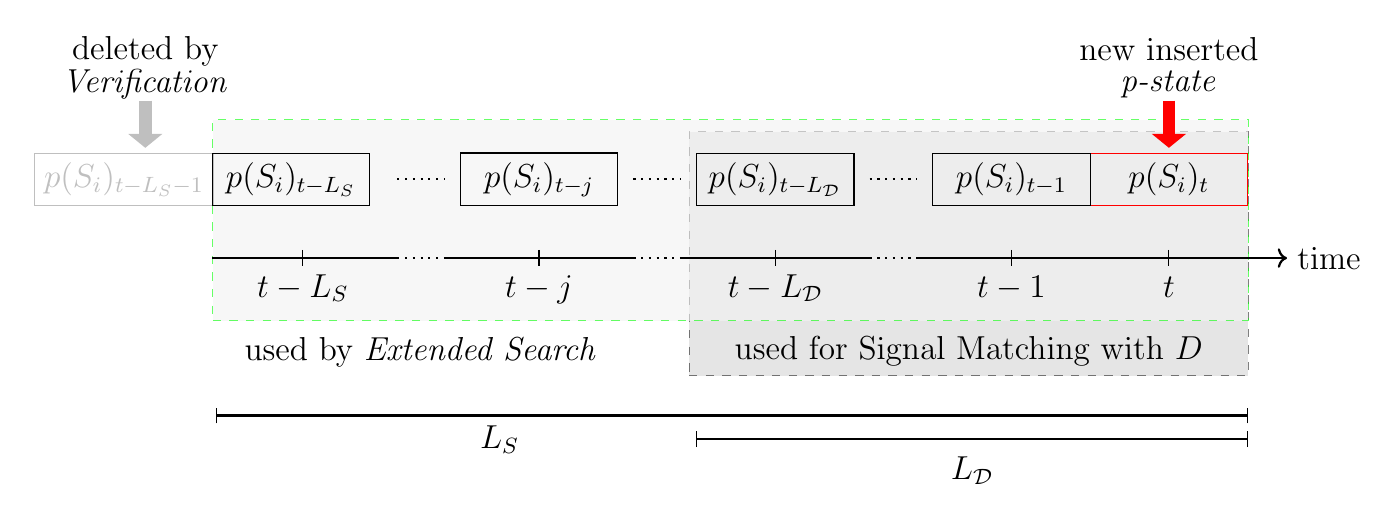
\begin{tikzpicture}\label{seq_buffer_length_tikz}
    
    \node (SignalMatcher) [rectangle, dashed, draw,
    fill = gray!40,
    opacity=0.5,
    minimum width=71.mm, minimum height=3.1cm, anchor= south west] at (6.9,-1.5) {};
    \node[anchor=south] at (SignalMatcher.south) {\large{used for Signal Matching with $D$}}; 

    \node (poly) [rectangle, dashed, draw,color=green,
    fill = gray!10,
    opacity=0.6,
    minimum width=131.5mm, minimum height=2.55cm, anchor= south west] at (0.85,-0.8) {};

    \draw[thick, ->] (9.8,0) -- (14.5,0) node[right]{\large time};
    \draw[thick, -, dotted] (9.2,0) -- (9.8,0);
    \draw[thick, -, dotted] (9.2,1) -- (9.8,1);
    \draw[thick, -] (6.8,0) -- (9.2,0);
    \draw[thick, -, dotted] (6.2,0) -- (6.8,0);
    \draw[thick, -, dotted] (6.2,1) -- (6.8,1);
    \draw[thick, -] (3.8,0) -- (6.2,0);
    \draw[thick, -] (0.85,0) -- (3.2,0);
    \draw[thick, -, dotted] (3.2,1) -- (3.8,1);
    \draw[thick, -, dotted] (3.2,0) -- (3.8,0);

    \draw[thick, -] (0.9,-2) -- (14,-2);
    \draw (0.9 cm,-2.1) -- (0.9cm,-1.9);    
    \draw (14 cm,-2.1) -- (14cm ,-1.9);

    \draw[thick, -] (7,-2.3) -- (14,-2.3);
    \draw (7 cm,-2.4) -- (7cm,-2.2);    
    \draw (14 cm,-2.4) -- (14cm ,-2.2);

    \node at (10.5, -2.7) {\large$L_{\mathcal{D}}$};
    \node at (4.5, -2.3) {\large$L_S$};
    \node at (3.5, -1.2) {\large{used by \emph{Extended Search}}};


    \draw (13,3pt) -- (13,-3pt);
    \draw (11 cm,3pt) -- (11 cm,-3pt);
    \draw (8 cm,3pt) -- (8 cm,-3pt);
    \draw (5 cm,3pt) -- (5 cm,-3pt);
    \draw (2 cm,3pt) -- (2 cm,-3pt);
    
    \foreach \x/\descr in {2/t-L_S,5/t-j,8/t-L_{\mathcal{D}},13/t,11/t-1}
    \node[font=\small, text height=1.75ex,
    text depth=.5ex] at (\x,-.4) {\large$\descr$};
    

    \draw[-{Triangle[width=12pt,length=5pt]}, line width=4.5pt, color=red](13, 2.) -- (13, 1.4);
    \node at (13,2.4) {
        \begin{small}
        \begin{tabular}{c}
            {\large{new inserted}}\\
            \large{\ps{}}
          \end{tabular}
        \end{small}
    };


    \node[rectangle,draw, minimum width = 2cm, 
    minimum height = 0.5, color=red, text=black] (r) at (13,1) {\large$p(S_i)_t$};
    \node[rectangle,draw, minimum width = 2cm, 
    minimum height = 0.5] (r) at (11,1) {\large$p(S_i)_{t-1}$};
    \node[rectangle,draw, minimum width = 2cm, 
    minimum height = 0.5] (r) at (8,1) {\large$p(S_i)_{t-L_{\mathcal{D}}}$};
    \node[rectangle,draw, minimum width = 2cm, minimum height = 0.4, color=lightgray, text=lightgray] (r) at (-0.27,1) {\large$p(S_i)_{t-L_{S}-1}$};
    \node[rectangle,draw, minimum width = 2cm, 
    minimum height = 0.5] (r) at (1.85,1) {\large$p(S_i)_{t-L_{S}}$};
    \node[rectangle,draw, minimum width = 2cm, 
    minimum height = 0.5] (r) at (5,1) {\large$p(S_i)_{t-j}$};

    \draw[-{Triangle[width=12pt,length=5pt]}, line width=4.5pt, color=lightgray](0,2.) -- (0, 1.4);
    \node at (0,2.4) {
        \begin{small}
        \begin{tabular}{c}
            {\large{deleted by}}\\
            \large{\textit{Verification}}
          \end{tabular}
        \end{small}
    };


\end{tikzpicture}}
  \vspace{-3mm}
  \caption{\ts{} containing multiple \emph{p-states}. Red rectangle: new \ps{} inserted at timestamp $t$. Green rectangle: Maximal length $L_S$ of \ts{}. \emph{Verification} method removes \ps{} surpassing $L_S$.}
  \label{figamtbuffer_detailed}
\end{figure}
\begin{figure}[ht]
  \centering
  \vspace{-8pt}
  \subfloat[]{\scalebox{0.6}{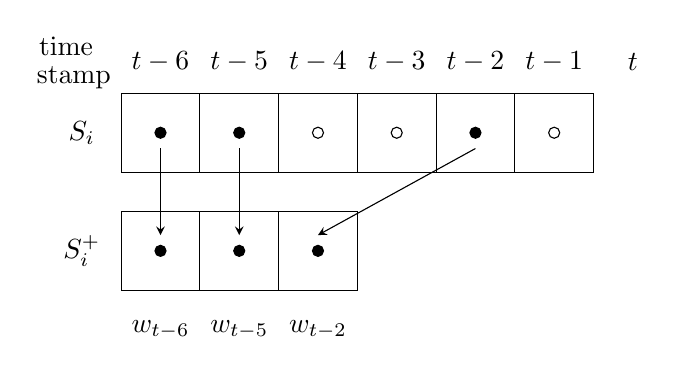
\begin{tikzpicture}
    
    \draw (2,9) rectangle ++(1,1);
    \draw (3,9) rectangle ++(1,1);
    \draw (4,9) rectangle ++(1,1);
    \draw (5,9) rectangle ++(1,1);
    \draw (6,9) rectangle ++(1,1);
    \draw (7,9) rectangle ++(1,1);

    \filldraw[black] (2.5,9.5) circle (2pt);
    \filldraw[black] (3.5,9.5) circle (2pt);
    \draw[black][black] (4.5,9.5) circle (2pt);
    \draw[black] (5.5,9.5) circle (2pt);
    \filldraw[black] (6.5,9.5) circle (2pt);
    \draw[black] (7.5,9.5) circle (2pt);
        

    \draw [-stealth](2.5,9.3) -- (2.5,8.2);
    \draw [-stealth](3.5,9.3) -- (3.5,8.2);
    \draw [-stealth](6.5,9.3) -- (4.5,8.2);

    \draw [] (4,7.5) rectangle ++(1,1);
    \draw [] (2,7.5) rectangle ++(1,1);
    \draw [] (3,7.5) rectangle ++(1,1);

    \filldraw[black] (4.5,8) circle (2pt);
    \filldraw[black] (2.5,8) circle (2pt);
    \filldraw[black] (3.5,8) circle (2pt);

    \node [] at (4.5,7) {$w_{t-2}$};
    \node [] at (2.5,7) {$w_{t-6}$};
    \node [] at (3.5,7) {$w_{t-5}$};

    \node at (1.5,9.5) {$S_{i}$};
    \node [] at (1.5,8) {$S^{+}_{i}$};

    \node at (1.3,10.6) {time};
    \node at (1.4,10.2) {stamp};
    \node at (8.5,10.4) {{$t$}};
    \node at (7.5,10.4) {{$t-1$}};
    \node at (6.5,10.4) {{$t-2$}};
    \node at (5.5,10.4) {{$t-3$}};
    \node at (4.5,10.4) {{$t-4$}};
    \node at (3.5,10.4) {{$t-5$}};
    \node at (2.5,10.4) {{$t-6$}};
\end{tikzpicture}}%
  \label{figamtextended_search}}
  \hfil
  \subfloat[]{\scalebox{0.2}{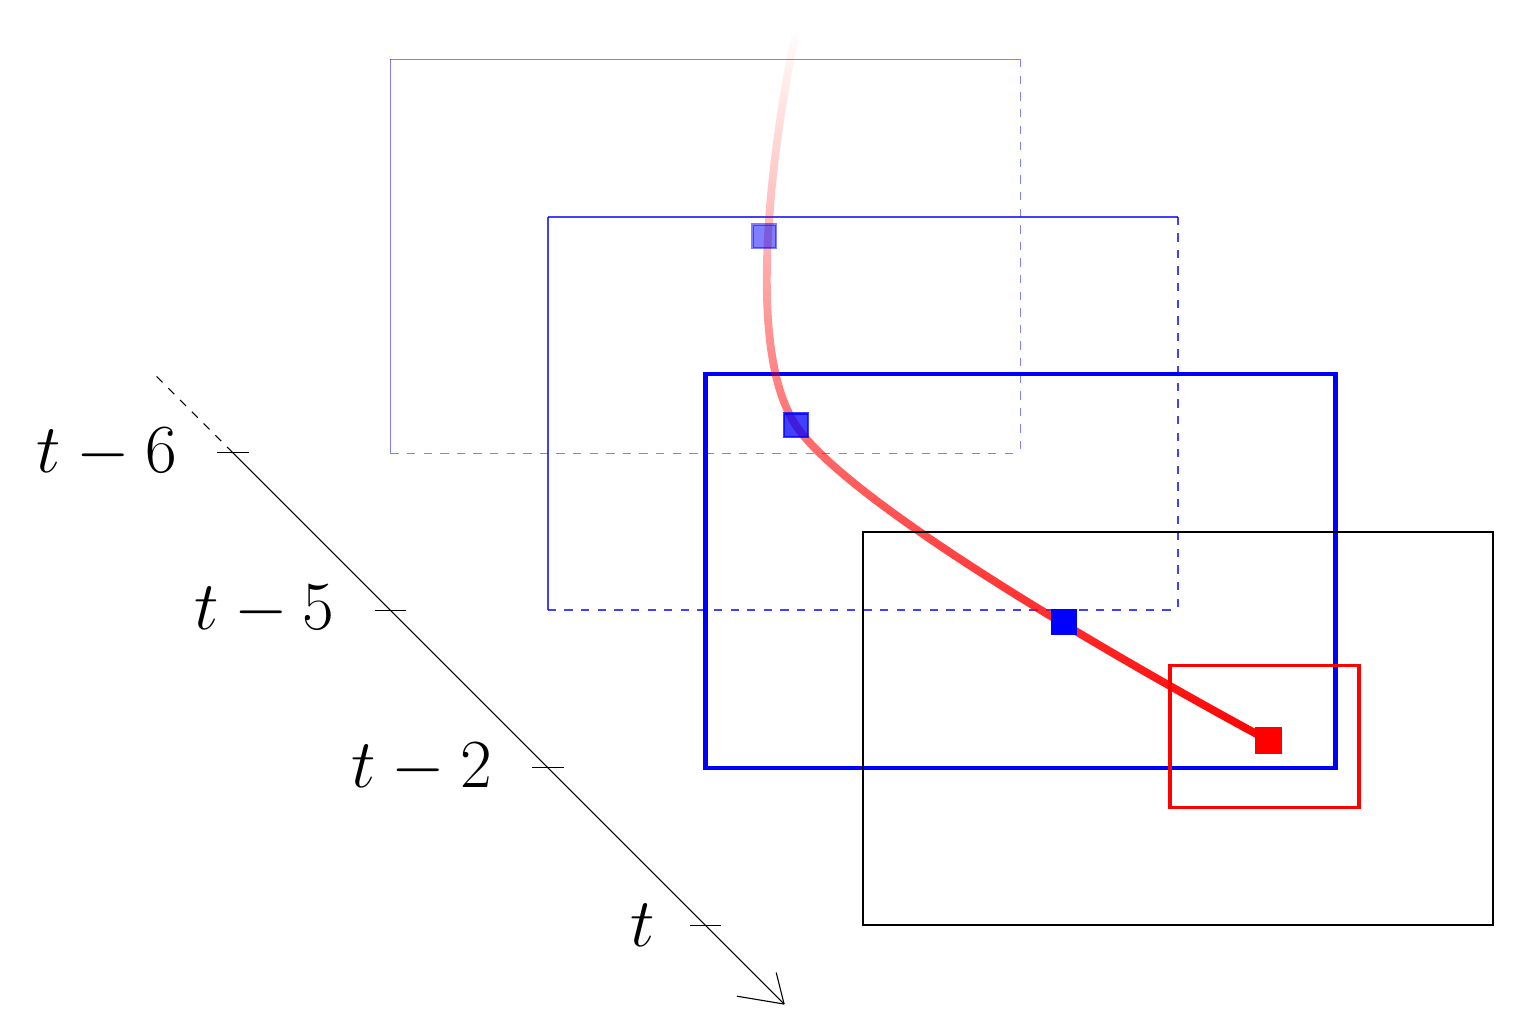
\begin{tikzpicture}

    \draw [blue,ultra thick] (0,0) rectangle ++(8,5);
    
    
    \draw [black,] (-6,4) -- (1,-3);
    \draw [black,dashed] (-6,4) -- (-7,5);
    
    \draw [black,] (1,-3) -- (0.9,-2.6);
    \draw [black,] (1,-3) -- (0.4,-2.9);
    
    \draw [black,] (-6.2,4) -- (-5.8,4);
    \draw [black,] (-4.2,2) -- (-3.8,2);
    \draw [black,] (-2.2,0) -- (-1.8,0);
    \draw [black,] (-0.2,-2) -- (.2,-2);
    
    \node at (-.8,-2) 
      {\Huge $t$};
    \node at (-3.6,0) 
      {\Huge $t-2$};
    
    \node at (-5.6,2) 
      {\Huge $t-5$};
    \node at (-7.6,4) 
      {\Huge $t-6$};
    
    \draw [blue,opacity=0.5,very thin](-4,4) -- (-4,9);
    \draw [blue,opacity=0.5,very thin](4,9) -- (-4,9);
    \draw [blue,opacity=0.5,very thin,dashed](4,9) -- (4,4);
    \draw [blue,opacity=0.5,very thin,dashed](-4,4) -- (4,4);
    \draw [blue, opacity=0.75,thick](-2,2) -- (-2,7);
    \draw [blue, opacity=0.75,thick](6,7) -- (-2,7);
    \draw [blue, opacity=0.75,thick,dashed](6,7) -- (6,2);
    \draw [blue, opacity=0.75,thick,dashed](-2,2) -- (6,2);
    \draw [line width=0.1cm ,red, path fading=north, fading angle=0] plot [smooth, tension=0.5] coordinates { (1.15, 9.35 ) (1.15,4.35) (7.15,0.35)};
    \draw [blue, opacity=0.50, thick, fill] ( 0.6, 6.6 ) rectangle ++ (0.3,0.3);
    \draw [blue, opacity=0.75, thick, fill] ( 1, 4.2 ) rectangle ++ (0.3,0.3);
    \draw [blue, thick,fill] ( 4.4, 1.7 ) rectangle ++ (0.3,0.3);
    \draw [opacity=1,very thick, fill, red] ( 7, 0.2 ) rectangle ++ (0.3,0.3);
    \draw [opacity=1,very thick, red] ( 5.9, -0.5 ) rectangle ++ (2.4, 1.8);
    \draw [thick] (2,-2) rectangle ++(8,5);
    
    
\end{tikzpicture}}%
  \label{figamtextended_search_2}}
  \caption{(a) The \emph{Extended Search} selects all \emph{p-states} of a \ts{} with value `1'. (b) Past images (blue) with pixel locations of $S_i^+$ and polynomial regression (red) with its search window in the image at timestamp $t$.}
  \label{fig_sim}
  \vspace{-15pt}
\end{figure}
A \ts{} in the $i$-th row of \B{} is denoted by $S_i$, and the \ps{} in $S_i$ at timestamp $t-j$ (with $j$ timestamps before the last image capture at $t$) is written as $p(S_i)_{t-j}$.
When a new association between $S_i$ and an \emph{image-point} in $\mathcal{P}_t$ is found, the \emph{image-point} is appended as a \ps{} at the end of $S_i$ (see red rectangles in Figs. \ref{figamtbuffer} and \ref{figamtbuffer_detailed}).

B{} uses two boundaries to cope with its dynamic nature: one limits the maximum number of rows, controlling the number of allowed \ts{} in the buffer, while the other restricts the maximum columns ($L_S$), defining the maximum length of a \ts{} in \B{}.
The limitation on rows serves as a safety measure to prevent memory overflow. It also counteracts the continuous insertion of new \ts{} into \B{} in noisy background conditions (e.g. sun reflections on water surfaces), making associations infeasible.
The maximum number of columns, corresponding to the number of \emph{p-states} per \ts{}, is primarily defined by the metrics used in the \emph{Extended Search} (Fig. \ref{figamtbuffer_detailed}).

\subsection{Local Search}\label{subsecamtlocal_search}
The \emph{Local Search} matches \ts{} in \B{} and \emph{image-points} in $\mathcal{P}_t$ based on the maximal linear movement $(\Delta px_{m}=(\Delta x_m,\Delta y_m))$ of a blinking marker between two consecutive frames, with $\Delta x_m$ and $\Delta y_m$ describing horizontal and vertical displacements, respectively.
The maximal expected displacement of a blinking marker between two frames, in pixel units, is defined as:
\begin{align}
\Delta px_{m} = 
(\lceil v_{x,\max}/f \rceil, \lceil v_{y,\max}/{f}\rceil)\label{eqamtlocal_search},
\end{align}
where $v_{x,\max}$ and $v_{y,\max}$ are the maximum horizontal and vertical velocities of a blinking marker in the image, respectively, and are measured in pixels per second over a one-second interval.
These values were experimentally determined by analyzing marker motion across frames under varying robot speeds, distances, and relative motion.

For each \ts{} in \B{}, the \emph{Local Search} constructs a fixed search area around the last inserted \ps{} using equation \eqref{eqamtlocal_search}.
For $S_i$, this search area is denoted by $p(S_i)_{t-1}\pm \Delta px_{m}$.
If an \emph{image-point} $p_{t,k}$ in $\mathcal{P}_t$ lies in the search area of $S_i$, $p_{t,k}$ is appended to $S_i$ as a new \ps{}.

This fixed search area works well when the relative movement between the \gls{RX} and \glsentryshort{TX} causes minimal marker displacement in the image, but it may be insufficient when a \gls{UAV} performs agile maneuvers.
The \emph{image-points} of $\mathcal{P}_t$ with unsuccessful insertion into \B{} by the \emph{Local Search} are stored in the subset $\mathcal{P}_t^*$. The subset of \B{}, denoted by \BS{}, stores all \ts{} with unsuccessful correspondence search by the \emph{Local Search}.
\BS{} and $\mathcal{P}_t^*$ are then used in the \emph{Extended Search}.

\subsection{Extended Search}\label{subsecamtextended_search}
The \emph{Extended Search} executes a correspondence search between the \ts{} in \BS{} and the \emph{image-points} in $\mathcal{P}_t^*$.
In \BS{}, it selects for each \ts{} only the \enquote*{$1$}-\emph{p-states} (blinking marker turned \enquote{on}; Fig. \ref{figamtextended_search}), resulting in a discontinuous, shorter \ts{}, denoted by $S_i^+$.
During the \enquote*{$1$}-\emph{p-states} the pixel coordinates of the marker are known with a higher precision compared to the \enquote*{$0$}-\emph{p-states} (blinking marker turned \enquote{off}).
On $S_i^+$, a weighted polynomial regression is performed by assigning individual weights to each \ps{} in $S_i^+$ using a time-dependent exponential decay function \cite{serwayModernPhysics2005}.
Applying a numerically stable \emph{QR}-Decomposition using \emph{Householder}-reflections \cite{golubMatrixComputations1996} solves the weighted least squares problem, avoiding computationally expensive and potentially numerically unstable matrix inversion \cite{ComputationalAlgorithmsFitting2003}.
The polynomial regression predicts the pixel coordinates $\hat{x}$ and $\hat{y}$ for timestamp $t$ and is denoted by $\hat{p}(S_i)_t$, for the blinking marker represented by $S_i$.
For each \ts{} in \BS{}, an individual search window is constructed based on the uncertainty in computing the regression coefficients, referred to as the prediction interval for a new response \cite{rossChapterRegression2014}.
With the Student's \texttt{t}-distribution (\texttt{t}$_{1-\frac{\alpha}{2},\nu}$), the search area around $\hat{p}{(S_i)_t}$ for timestamp $t$ is defined by:
\begin{align}
  \hat{p}(S_i)_t \pm (\text{\texttt{t}}_{1-\frac{\alpha}{2},\nu})\sqrt{\hat{\sigma}_w^2\left(1+\frac{1}{L_i^+}+\frac{(t-\bar{t}_w)^2}{\sum_{k=1}^{L_i^+}{(t_k-\bar{t}_w)^2}}\right)},\label{eqamtextended_search}
\end{align}
where $\hat{\sigma}_w^2$ denotes the unbiased estimator for the error variance $\sigma_w$. $\bar{t}_w$ represents the weighted mean of all timestamps in $S_i^+$, with weights determined by an exponential decay function.
$L_i^+$ is the number of \emph{p-states} in $S_{i}^+$, $\alpha$ is the desired probability for the critical value from the Student's \texttt{t}-distribution, and $\nu$ is its degree of freedom, defined by:
\begin{align}
  \nu = L_i^+ - (d + 1),
\end{align}
where $d$ denotes the polynomial degree.

The maximum permissible length of a \ts{} in \B{}, denoted by $L_S$, depends on the parameters of the \emph{Extended Search}. 
The desired polynomial degree $d$, crucial for approximating the past movement of a blinking marker, is influenced by the quantity of past \emph{p-states} stored in a \ts{}. 
Consequently, a larger $L_S$ entails accounting for a longer historical trajectory, requiring a higher polynomial degree, and vice versa.
This relationship can be expressed by:
\begin{align}
L_S = \eta d\label{eqamtseq_length},
\end{align}
where $d$ is the polynomial degree for the regression and $\eta \in \mathbb{N}^+$ is a parameter chosen through experiments.

Similarly to the \emph{Local Search}, if an \emph{image-point} from $\mathcal{P}_t^*$ lies in the search window of a \ts{}, defined by equation \eqref{eqamtextended_search}, it is appended to the end of that \ts{}.
The \emph{image-points} from $\mathcal{P}_t^*$ for which the \emph{Extended Search} did not find a correspondence in \B{}$^*$ are stored in a new set, denoted $\mathcal{P}_t^\Gamma$. 
Similarly, \emph{t-series} from \B{}$^*$ without new insertions from $\mathcal{P}_t^*$ are stored in a new set, \B{}$^\Gamma$.

\begin{figure*}[!t]
  \centering
  \subfloat[\label{fig:eval:two_tx}]{
    \scalebox{1.1}{\begin{tikzpicture}
    % \clip (0.5,0) rectangle ++ (8.6,3);     
    \node[anchor=south west,inner sep=0] (a) at (0,0) { 
    \includegraphics[width=0.45\textwidth]{stand_cam_2.png}};
    
    \begin{scope}[x={(a.south east)},y={(a.north west)}]

             
      \node [black] at(0.1, 0.5) {\glsentryshort{RX}};
      \node [black] at(0.5, 0.48) {\glsentryshort{TX}1};
      \node [white] at(0.82, 0.12) {\glsentryshort{TX}2};

    \end{scope}
  \end{tikzpicture}
}
  } 
  \subfloat[\label{fig:eval:overview_graph}]{
    \scalebox{0.4}{\section{Experimental setup}\label{sec:exp_setup}

This section details the setup of human experiments, including the dataset, the criteria for selecting systems to be evaluated, and the process for assigning tasks among annotators.

\subsection{Dataset and language pairs}

The human annotation experiments are performed on the system outputs from the news domain in WMT2023 \citep{freitag-etal-2023-results}, covering two language pairs: Chinese to English (\ZhEn) and English to German (\EnDe). Basic statistics are in \tableref{tab:basic_stats}.

\sisetup{table-text-alignment=center,table-format=6.0}
\begin{tabular}{lSSSSrrS}
\toprule
{\textbf{Attribute}} & {\textbf{Declarations}} & {\textbf{Users}} & {\textbf{Inactive Users}} & {\textbf{Ambiguous Users}} & \multicolumn{2}{c}{\textbf{Class Proportion}} & {\textbf{Subreddits}} \\
\midrule
Year of Birth & 420803 & 401390 & 1630 & 17341 & Old: 56.19\% & Young: 43.81\% & 9806 \\
Gender & 424330 & 403428 & 1634 & 18337 & Male: 50.89\% & Female: 49.11\% & 9809 \\
Partisan Affiliation & 6369 & 6118 & 4 & 251 & Dem.: 54.55\% & Rep.: 45.45\% & 9137 \\
\bottomrule
\end{tabular}


\subsection{System pairs}\label{sec:sys_pairs}

Due to the time and cost involved in human evaluation, pairwise comparisons of all MT systems in the \sxs~settings are impractical. Therefore, 5 system pairs are selected per language pair (\tableref{tab:sys_pairs}), which are drawn from the systems in the WMT 2023 General Machine Translation Task \citep{kocmi-etal-2023-findings}.%, with a focus on systems with similar quality, as distinguishing systems with smaller quality differences presents a greater challenge in practical scenarios. 
% , focusing on systems with similar quality, as distinguishing between systems with smaller quality differences presents a greater challenge in practical scenarios.

\begin{table}[ht]
\fontsize{7}{8}\selectfont
\centering
% \renewcommand{\arraystretch}{0.8} % Reduce vertical space
\resizebox{0.92\columnwidth}{!}{%
\begin{tabular}{@{}p{0.1cm}p{1.51cm}cp{0.3cm}p{0.4cm}p{2.1cm}@{}}
\midrule
        & \textbf{System Pairs} & \textbf{Rank} & \textbf{\textit{p}} &  \textbf{Cross-BLEU} & \textbf{Criteria} \\ \midrule
\multirow{10}{*}{\rotatebox{90}{\ZhEn}} & GPT4-5shot &  1  & \multirow{2}{*}{0.05} & \multirow{2}{*}{62.2} & \multirow{2}{*}{Top 2 systems} \\
                                       & Lan-BridgeMT & 2 & & & \\\cmidrule{2-6}
                                       & HW-TSC & 4 & \multirow{2}{*}{0.27} & \multirow{2}{*}{57.3} & \multirow{4}{*}{High text similarity} \\
                                       & ONLINE-A & 5 & & & \\\cmidrule{2-5}
                                       & IOL-Research & 6  & \multirow{2}{*}{0.17} & \multirow{2}{*}{52.2} & \\
                                       & ONLINE-B & 8 & & & \\\cmidrule{2-6}
                                       & ONLINE-W & 10 & \multirow{2}{*}{0.10} & \multirow{2}{*}{31.2} & \multirow{4}{*}{Lower text similarity} \\
                                       & NLLB\_Greedy & 12 & & & \\\cmidrule{2-5}
                                       & NLLB\_BLEU & 14 & \multirow{2}{*}{0.40} & \multirow{2}{*}{35.7} & \\
                                       & ONLINE-M & 15 &  & & \\\midrule
\multirow{10}{*}{\rotatebox{90}{\EnDe}} & ONLINE-W  & 1   & \multirow{2}{*}{0.09} & \multirow{2}{*}{53.1} & \multirow{2}{*}{Top 2 Systems} \\  
                                       & GPT4-5shot  & 2  & & & \\\cmidrule{2-6}
                                       & ONLINE-Y   & 5   & \multirow{2}{*}{0.48} & \multirow{2}{*}{62.0} &  \multirow{4}{*}{High text similarity}\\
                                       & ONLINE-A   & 6   & & & \\\cmidrule{2-5}
                                       & ONLINE-M   & 7   & \multirow{2}{*}{0.22} & \multirow{2}{*}{56.3} & \\
                                       & ONLINE-G   & 8   & & & \\\cmidrule{2-6}
                                       & GPT4-5shot & 2  & \multirow{2}{*}{0.11} & \multirow{2}{*}{39.3} & \multirow{4}{*}{Lower text similarity} \\
                                       & refA       & 3   & & & \\\cmidrule{2-5}
                                       & NLLB\_BLEU & 10 & \multirow{2}{*}{0.24} & \multirow{2}{*}{44.3} & \\
                                       & Lan-BridgeMT  & 11 & & & \\\midrule
\end{tabular}%
}
\caption{Systems annotated in the human experiments. The ranks are determined by XCOMET. The $p$ values are calculated by a random permutation test with 10000 trials to determine quality similarity. Cross-BLEU quantifies the text similarity of system outputs.
}
\label{tab:sys_pairs}
\vspace{-3pt}
\end{table}

Two features are considered when forming system pairs: text similarity and quality similarity. For text similarity, cross-BLEU \citep{papineni-etal-2002-bleu} is applied. For quality similarity, XCOMET-QE-Ensemble (XCOMET) \citep{xcomet, freitag-etal-2023-results} is used in tandem with a random permutation test.\footnote{\texttt{permutation\_test} from \texttt{scipy.stats}.} XCOMET provides segment scores for each system. Two systems are considered similar in quality if the permutation test of their segment scores returns $p > 0.05$. 
% \url{https://docs.scipy.org/doc/scipy-1.14.1/reference/generated/scipy.stats.permutation_test.html}

For each language pair, the top two systems identified by XCOMET form a pair; two pairs have high text similarity (cross-BLEU); and two have low text similarity. In all cases, systems with similar quality were selected, as distinguishing small quality differences presents a greater challenge in practical scenarios. The system pairs are listed in \tableref{tab:sys_pairs}.\footnote{For brevity, NLLB\_MBR\_BLEU is referred to as NLLB\_BLEU in this work.} Applying these criteria resulted in GPT4-5shot appearing twice in \EnDe. This has the benefit of allowing comparison between each instance of this system's evaluation in the side-by-side settings.%~to examine whether a system's MQM score varies with different comparison systems.

\subsection{Task assignment}\label{sec:task_assignment}

The annotation experiments are conducted by professional translators who regularly perform MQM annotation. Tasks are distributed approximately evenly among 8 annotators for \ZhEn~ and 10 for \EnDe. To mitigate rater bias, we use the within-subject setup of \citet{riley-etal-2024-finding}: for each input document, all system translations for that document are evaluated by the same set of 3 annotators. Additionally, each translation is evaluated by the same 3 annotators in all 3 annotation settings.
%each input document is evaluated by the same annotator across all settings. Three rounds of human annotation are conducted for each setting. In each round, task assignments are ``rotated'', with tasks assigned to annotator 1 in round 1 given to annotator 2 in round 2, and so on. The same task assignments are used across all three settings in each round.

% \subsection{Score calculation}\label{sec:result_score_calc}

% Annotations from the expert annotators are converted to numeric scores for system and annotation setting comparison. For both \psxsmqm~and \sxsmqm, the segment score is the average of the scores assigned by each annotator, with each score determined by the error severity and category. Gibberish segments score 25 points without further error annotation; major errors are penalized by 5 points, minor punctuation errors by 0.1, and other minor errors by 1. The system score is obtained by averaging the segment scores. MQM scores are the lower the better, with an error-free segment receiving a score of 0.

% \begin{table}[ht]
% \fontsize{6}{7}\selectfont
% \centering
% % \renewcommand{\arraystretch}{0.8} % Reduce vertical space
% \resizebox{0.55\columnwidth}{!}{%
% \begin{tabular}{@{}p{0.55cm}p{1.6cm}p{0.7cm}@{}}
% \midrule
% \textbf{Severity}   & \textbf{Category} & \textbf{Weight} \\ \midrule
% \multirow{2}{*}{\major}  & Non-translation & 25  \\
%                          & Others   & 5 \\\cmidrule{1-3}
% \multirow{2}{*}{\minor}  & Fluency/Punctuation & 0.1  \\
%                          & Others   & 1 \\\midrule
% \end{tabular}%
% }
% \caption{MQM error span weighting scheme. Gibberish segments score 25 points, \major~errors 5 points, and \minor~errors 1 point, except for \minor~punctuation errors, which are weighted at 0.1 point each.
% }
% \label{tab:weighting-scheme}
% \end{table}

% The scoring of \sxsqr~follows MQM in that a lower score is better. In each rated pair, the \texttt{much worse} translation segment                is penalized by 2 points, and the \texttt{worse} segment by 1 point. If both translations are of similar quality, no penalty is applied. As the MQM settings, the segment score is the average of the scores assigned by each annotator. The system score is averaged over the segment scores.

% \begin{table}[ht]
% \fontsize{5}{6}\selectfont
% \centering
% % \renewcommand{\arraystretch}{0.8} % Reduce vertical space
% \resizebox{0.55\columnwidth}{!}{%
% \begin{tabular}{@{}p{1.5cm}p{0.7cm}@{}}
% \midrule
% \textbf{Category} & \textbf{Weight} \\ \midrule
% Much worse & 2  \\
% Worse      & 1  \\
% About the same & 0 \\\midrule
% \end{tabular}%
% }
% \caption{\sxsqr~segment scoring scheme.
% }
% \label{tab:weighting-scheme-qr}
% \vspace{-10pt}
% \end{table}

}}
    \caption{(a) Two \glsentrylongpl{TX} flying in front of one \glsfirst{RX}. 
    (b) Experimental Setup:
    In experiments 2-6, the right camera (red) of the \gls{RX} points at two \glsentryshortpl{TX} flying parallel to the $y$-axis.
    In Experiment 7, only one \gls{TX} is used to test the algorithm during agile maneuvers.
    Numbers around the \glsentryshortpl{TX}' arms show the \gls{LED}-IDs emitted by the blinking markers.}
    \label{fig:eval:overview}
    \vspace*{-10pt}
\end{figure*}
\subsection{Verification}\label{subsecamtverification}
The \emph{Verification} method contains multiple tasks.
If \B{}$^\Gamma$ contains \ts{}, both correspondence searches failed to find new associations for the stored \ts{} in \B{}$^\Gamma$. 
\begin{figure}[!b]
  \centering
  \vspace{-5pt}
  \scalebox{0.45}{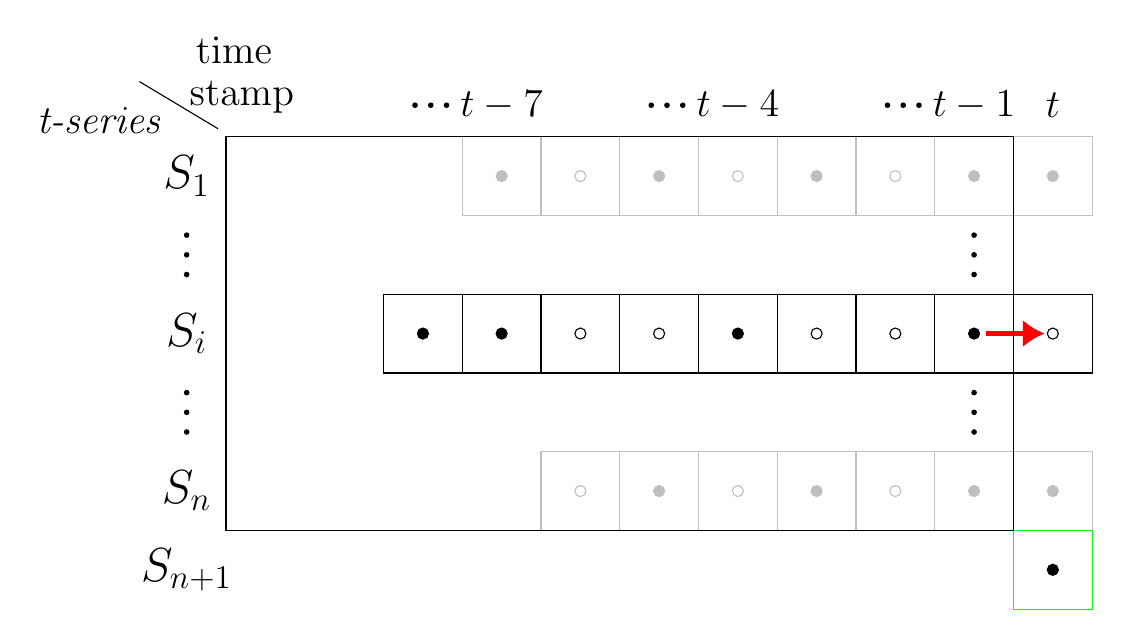
\begin{tikzpicture}
    \draw[lightgray] (3,13) rectangle ++(1,1);
    \draw[lightgray] (4,13) rectangle ++(1,1);
    \draw[lightgray] (5,13) rectangle ++(1,1);
    \draw[lightgray] (6,13) rectangle ++(1,1);
    \draw[lightgray] (7,13) rectangle ++(1,1);
    \draw[lightgray] (8,13) rectangle ++(1,1);
    \draw[lightgray] (9,13) rectangle ++(1,1);
    \draw[lightgray] (10,13) rectangle ++(1,1);

    \draw(2,11) rectangle ++(1,1);
    \draw(3,11) rectangle ++(1,1);
    \draw(4,11) rectangle ++(1,1);
    \draw(5,11) rectangle ++(1,1);
    \draw(6,11) rectangle ++(1,1);
    \draw(7,11) rectangle ++(1,1);
    \draw(8,11) rectangle ++(1,1);
    \draw(9,11) rectangle ++(1,1);
        
    \filldraw (9.5,12.75) circle (0.8pt);
    \filldraw (9.5,12.5) circle (0.8pt);
    \filldraw (9.5,12.25) circle (0.8pt);
    
    \filldraw (9.5,10.75) circle (0.8pt);
    \filldraw (9.5,10.5) circle (0.8pt);
    \filldraw (9.5,10.25) circle (0.8pt);
    
    \draw[ lightgray] (4,9) rectangle ++(1,1);
    \draw[ lightgray] (5,9) rectangle ++(1,1);
    \draw[ lightgray] (6,9) rectangle ++(1,1);
    \draw[ lightgray] (7,9) rectangle ++(1,1);
    \draw[ lightgray] (8,9) rectangle ++(1,1);
    \draw[ lightgray] (9,9) rectangle ++(1,1);
    \draw[ lightgray] (10,9) rectangle ++(1,1);
    
    \filldraw[black] (2.5,11.5) circle (2pt);
    \filldraw[black] (3.5,11.5) circle (2pt);
    \draw[black][black] (4.5,11.5) circle (2pt);
    \draw[black] (5.5,11.5) circle (2pt);
    \filldraw[black] (6.5,11.5) circle (2pt);
    \draw[black] (7.5,11.5) circle (2pt);
    \draw[black] (8.5,11.5) circle (2pt);
    \filldraw[black] (9.5,11.5) circle (2pt);
    
    \filldraw[lightgray] (3.5,13.5) circle (2pt);
    \draw[lightgray] (4.5,13.5) circle (2pt);
    \filldraw[lightgray] (5.5,13.5) circle (2pt);
    \draw[lightgray] (6.5,13.5) circle (2pt);
    \filldraw[lightgray] (7.5,13.5) circle (2pt);
    \draw[lightgray] (8.5,13.5) circle (2pt);
    \filldraw[lightgray] (9.5,13.5) circle (2pt);
    \filldraw[lightgray] (10.5,13.5) circle (2pt);


    \draw[lightgray] (4.5,9.5) circle (2pt);
    \filldraw[lightgray] (5.5,9.5) circle (2pt);
    \draw[lightgray] (6.5,9.5) circle (2pt);
    \filldraw[lightgray] (7.5,9.5) circle (2pt);
    \draw[lightgray] (8.5,9.5) circle (2pt);
    \filldraw[lightgray] (9.5,9.5) circle (2pt);
    \filldraw[lightgray] (10.5,9.5) circle (2pt);

    \node at (0.1, 15.1) [align=left] {\Large time};
    \node at (0.2, 14.5) [align=left] {\Large stamp};
    
    \node at (-1.6,14.2) [align=left] {\Large \ts{}};
    \draw (-.1,14.1) -- (-1.1,14.7);

    \node at (-0.5,13.5) {\LARGE$S_{1}$};
    \node at (9.5,14.4) {\Large{$t-1$}};
    \node at (6.5,14.4) {\Large{$t-4$}};

    \node at (3.5,14.4) {\Large{$t-7$}};
    \node at (10.5,14.4) {\Large{$t$}};
    
    \filldraw (8.8,14.4) circle (0.8pt);
    \filldraw (8.6,14.4) circle (0.8pt);
    \filldraw (8.4,14.4) circle (0.8pt);
    
    \filldraw (5.8,14.4) circle (0.8pt);
    \filldraw (5.6,14.4) circle (0.8pt);
    \filldraw (5.4,14.4) circle (0.8pt);

    \filldraw (2.8,14.4) circle (0.8pt);
    \filldraw (2.6,14.4) circle (0.8pt);
    \filldraw (2.4,14.4) circle (0.8pt);

    \filldraw (-0.5,12.75) circle (0.8pt);
    \filldraw (-0.5,12.5) circle (0.8pt);
    \filldraw (-0.5,12.25) circle (0.8pt);

    \filldraw (-0.5,10.75) circle (0.8pt);
    \filldraw (-0.5,10.5) circle (0.8pt);
    \filldraw (-0.5,10.25) circle (0.8pt);

    \draw[] (10,11) rectangle ++(1,1);
    \draw[black, ] (10.5,11.5) circle (2pt);

    \draw [ultra thick, red,-{Latex[length=2.8mm,width=3.5mm]} ](9.65,11.5) -- (10.4,11.5);
    \draw[green] (10,8) rectangle ++(1,1);
    \filldraw[black] (10.5,8.5) circle (2pt);
    \node [] at (-0.5,8.5) {\LARGE $S_{n+1}$};
    \node at (-0.5,11.5) {\LARGE $S_{i}$};
    \node at (-0.5,9.5) {\LARGE $S_{n}$};
    \draw (0,9) rectangle ++(10,5);

\end{tikzpicture}
}
  \caption{$S_1$ and $S_n$ in gray: successful correspondence searches by the \emph{Local Search} or \emph{Extended Search}. Red arrow: duplication of $p(S_i)_{t-1}$ to `$0$'-\ps{} at timestamp $t$. Green rectangle: initialization of a new \ts{} at the end of \B{}.} 
  \label{fig:verification}
\end{figure}
The \gls{AMT} approach expects that a blinking marker represented by the \ts{} in \B{}$^\Gamma$ is either \enquote{off} in the image frame at timestamp $t$ or otherwise not visible.
Consequently, for all \ts{} in \B{}$^\Gamma$, the pixel coordinates of the \emph{p-states} at timestamp $t-1$ are duplicated and inserted as new `$0$'-\emph{p-states}.
Since the \emph{Extended Search} ignores '0'-\ps{}, the previous motion is not considered when inserting the '0'-\ps{}.
In Fig. \ref{fig:verification}, a red arrow highlights this process for $S_i$.

This could result in continuously inserting \emph{p-states} representing `$0$' bits into \ts{} that lack new data associations.
This scenario is likely to occur when a blinking marker exits the \gls{FOV} of the camera or if it becomes occluded, both of which would result in a \ts{} containing only `0'-\emph{p-states}.
In the \emph{Verification} method, the validity of each \ts{} in \B{} confirms the condition
\begin{align}
  \sum_{j=t-(e+b_{m,0})}^{t} p_\texttt{s}(S_i)_j \geq e+b_{m,0}\label{eqamtverification} \hspace{1cm} \{i\in \mathcal{B}\},
\end{align}
with $p_\texttt{s}(S_i)_j$ denoting the \texttt{state} of $p(S_i)$ at timestamp $j$, and $e$ denoting the expected bit error rate per sequence transmission. 
If the condition \eqref{eqamtverification} is violated for a \ts{} due to continuous `$0$'-\ps{} insertions, the \emph{Verification} method deletes the \ts{} from \B{}.
To re-track a blinking marker after a tracking failure caused by situations such as obstruction by an object, the value of $e$ should be set sufficiently high to keep the invalid \emph{t-series} in the buffer.
This allows for re-tracking the blinking marker by the \emph{Extended Search}.
However, by increasing the value of $e$, the overall computational cost and memory usage increases since invalid \emph{t-series} are kept longer in \B{} until condition \eqref{eqamtverification} is violated.
Additionally, the \emph{Verification} method deletes the \emph{p-states} in a \ts{} that surpass the maximum number of columns, $L_S$, preventing memory overflow (Fig. \ref{figamtbuffer_detailed}).

Each \emph{image-point} in $\mathcal{P}_t^\Gamma$ is inserted as a new \ts{} into \B{}, thereby increasing the numbers of rows by the length of $\mathcal{P}_t^\Gamma$, allowing the algorithm to track newly appearing blinking markers in the \gls{FOV} of the camera.
Fig. \ref{fig:verification} depicts this process for a single \emph{image-point} by the green rectangle.

Consequently by this point, all \emph{image-points} in $\mathcal{P}_t$ have been inserted into \B{}, either by the \emph{Local Search}, \emph{Extended Search}, or \emph{Verification} method. 


\section{Experimental Evaluation}\label{sec:evaluation}
\begin{wrapfigure}{r}{0.25\textwidth}
    \scalebox{0.5}{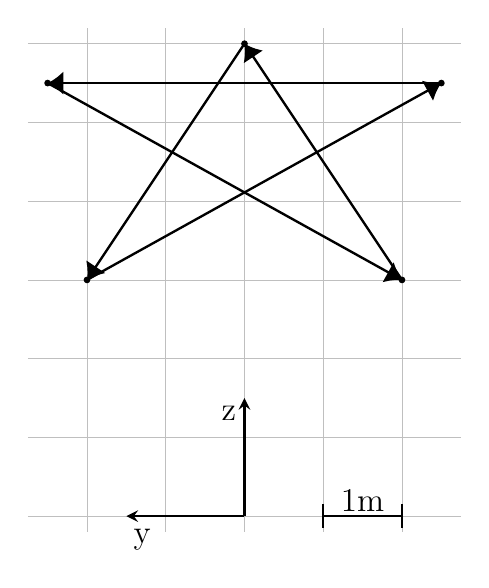
\begin{tikzpicture}[decoration = {markings,
  mark = at position 0.0 with {\arrow[>=stealth]{<}}
}
]
\draw[step=1cm,lightgray,very thin] (-2.75,-0.2) grid (2.75,6.2);


  \draw [line width=0.3mm, -] (1,0) -- (2.,0) ;
  \draw [line width=0.3mm, -] (1,-.15) -- (1,0.15) ;
  \draw [line width=0.3mm, -] (2,-0.15) -- (2,0.15) ;
  \node at (1.5,0.2) {\large 1m};

  \filldraw [] (0, 6) circle (1pt);
  \filldraw [] (2, 3) circle (1pt);
  \filldraw [] (-2, 3) circle (1pt);
  \filldraw [] (-2.5, 5.5) circle (1pt);
  \filldraw [] (2.5, 5.5) circle (1pt);

  \draw [line width=0.3mm, -{Latex[length=2mm,width=3mm]}] (0,6) -- (-2,3.);
  \draw [line width=0.3mm, {Latex[length=2mm,width=3mm]}-] (2.5,5.5) -- (-2,3.) ;
  \draw [line width=0.3mm, -{Latex[length=2mm,width=3mm]}] (2.5,5.5) -- (-2.5,5.5) ;
  \draw [line width=0.3mm, {Latex[length=2mm,width=3mm]}-] (2,3) -- (-2.5,5.5) ;
  \draw [line width=0.3mm, -{Latex[length=2mm,width=3mm]}] (2,3) -- (0,6) ;

  \draw [line width=0.3mm, -stealth] (0,0) -- (-1.5,0);
  \draw [line width=0.3mm, -stealth] (0,0) -- (0,1.5) ;
  \node at (-0.2,1.3) {\large z};
  \node at (-1.3,-0.3) {\large y};
\end{tikzpicture}
}
    \caption{$y$-$z$ coordinates for \glsentryshort{TX}1 and \glsentryshort{TX}2 during \enquote{star} trajectory in Exp. 6.} 
    \label{fig:eval:star}
    \vspace*{-10pt}
\end{wrapfigure}
We evaluated the \gls{AMT} approach in outdoor experiments, comparing it with the state-of-the-art \gls{4DHT} approach \cite{walterMutualLocalizationUAVs2018} used in the previous version of the \gls{UVDAR} system. 
A quadrotor \gls{UAV} based on the \emph{Holybro X500} platform was used with an \emph{Intel NUC 10 i7FNK} (6 cores, up to \SI{4.7}{\giga\hertz}; details in \cite{hertMRSDroneModular2023}).
Both onboard and offline executions showed indiscernible performance differences.
Therefore, we re-executed both algorithms on the same computer (\emph{Intel i7-8550U} CPU, \SI{1.8}{\giga\hertz}) and dataset for a fair comparison.
This paper presents the seven most relevant experiments from a set of 14 involving two/three \glspl{UAV} (Fig. \ref{fig:eval:overview}).
Each trajectory in each experiment was flown in a periodic loop, with a minimum duration of \SI{60}{\second}.

Exp. 1:  \gls{TX}1 and \gls{TX}2 hovered at distances of \SI{4.12}{\meter} and \SI{8.06}{\meter} from the \gls{RX}, respectively. 
The \gls{RX} rotated around its yaw axis, causing the blinking markers of the \glsentryshortpl{TX} to move in a linear horizontal trajectory within the image.

\begin{figure*}[!ht]
  \centering
\includegraphics[width=1.\textwidth]{exp_1.pdf}
  \caption{Experiment 1: Yaw angle ($\psi$) of \gls{RX} with extracted \gls{LED}-IDs.}
  \label{fig:eval:exp_1}
\end{figure*}
\begin{figure*}[!ht]
  \centering
\includegraphics[width=1.\textwidth]{exp_2.pdf}
  \caption{ 
  Experiment 2: Yaw angle ($\psi$) of \gls{RX} and \glsentryshortpl{TX} with extracted \gls{LED}-IDs.}
  \label{fig:eval:exp_2}
\end{figure*}
\begin{figure*}[!ht]
  \centering
\includegraphics[width=1.\textwidth]{exp_3.pdf}
  \caption{ 
  Experiment 3: Roll ($\phi$) and Pitch $(\theta)$ angle of \gls{RX} with extracted \gls{LED}-IDs.}
  \label{fig:eval:exp_3}
\end{figure*}
\begin{figure*}[!ht]
  \centering
    \includegraphics[width=\textwidth]{exp_4_5_6.pdf}
    \caption{Extracted \gls{LED}-IDs with y-coordinates for \glsentryshort{TX}1 and \glsentryshort{TX}2 in linear (Exp. 4; left), circular (Exp. 5; center), and \enquote{star} (Exp. 6; right) trajectories. Gray areas highlight when the \glsentryshortpl{TX} were close in the image.}
  \label{fig:eval:exp_4_5_6}
\end{figure*}
\begin{figure*}[!ht]
    \includegraphics[width=\textwidth]{exp_7.pdf}
    \caption{Experiment 7: Extracted \gls{LED}-IDs with a relative velocity of \gls{TX}1 during the fastest linear (left), circular (center), and \enquote{star} (right) trajectories.}
  \label{fig:eval:exp_7}
\end{figure*}

Exp. 2: All \glspl{UAV} followed a parallel linear trajectory of \SI{8}{\meter} (Fig. \ref{fig:eval:overview_graph}), with the \glsentryshortpl{TX} rotating 180 degrees and the \gls{RX} rotating between 0 and 90 degrees.
The rotations introduced additional horizontal movement and signal crosstalking when two blinking markers of one \glsentryshort{TX} were close in the image due to its rotation.

Exp. 3: Similar to Exp. 1, the \glspl{TX} hovered at minimum relative distances of \SI{4.12}{\meter} and \SI{8.06}{\meter} from the \gls{RX}, and at maximum relative distances of \SI{8.06}{\meter} and \SI{12.04}{\meter} from the \gls{RX} for \glsentryshort{TX}1 and \glsentryshort{TX}2, respectively.
The \gls{RX} followed a linear trajectory of \SI{4}{\meter} in the $x$-direction, causing vertical motion of the \glsentryshortpl{TX} markers in the image and testing the algorithm's response to abrupt deceleration and acceleration of the markers in the image.

Exp. 4: \glsentryshort{TX}1 and \glsentryshort{TX}2 followed linear trajectories of \SI{8}{\meter} perpendicular to the \gls{RX}'s camera optical axis.
\glsentryshort{TX}1 had a minimum relative distance of \SI{4}{\meter} and a maximum relative distance of \SI{5.66}{\meter}, while \glsentryshort{TX}2 had a minimum relative distance of \SI{8}{\meter} and a maximum relative distance of \SI{8.94}{\meter}, resulting in linear motion of the blinking markers in the image with sudden stops at the endpoints.
The maximum velocities of \glsentryshort{TX}1 and \glsentryshort{TX}2 were \SI{1.19}{\meter\per\second} and \SI{1.54}{\meter\per\second}, respectively.
This experiment also introduced occlusions of \glsentryshort{TX}2 by \glsentryshort{TX}1 at the center of their trajectories.

Exp. 5: The \glsentryshortpl{TX} followed circular trajectories, with \glsentryshort{TX}1 having a radius of \SI{1}{\meter}, a maximum velocity of \SI{0.6}{\meter\per\second}, and a relative distance of \SI{4.12}{\meter} from the \gls{RX}.
\glsentryshort{TX}2 had a radius of \SI{1.5}{\meter}, a maximum velocity of \SI{1.44}{\meter\per\second}, and a relative distance of \SI{8.14}{\meter} from the \gls{RX}.
This experiment evaluated the algorithm's performance on curved paths and during occlusions caused by \glsentryshort{TX}1, adding complexity when both \glsentryshortpl{TX} were close together in the image.

Exp. 6: The \glsentryshortpl{TX} followed a \enquote{star} trajectory (Fig. \ref{fig:eval:star}), with \glsentryshort{TX}1 at \SI{4}{\meter} and \glsentryshort{TX}2 at \SI{8}{\meter} distance along the $x$-axis, resulting in the most complex motions in the image. 
\glsentryshort{TX}1's maximum velocity was \SI{2.22}{\meter\per\second}, while \glsentryshort{TX}2's was \SI{1.63}{\meter\per\second}.

Exp. 7: In this experiment, \gls{TX}1 was the only transmitter. We flew similar trajectories to Exp. 4-6 at two different speeds to evaluate the \gls{AMT} approach for agile multi-robot systems. 
For the linear trajectory, \gls{TX}1 reached relative maximum speeds of \SI{2.40}{\meter\per\second} and \SI{5.43}{\meter\per\second}; for the circular trajectory, \SI{2.57}{\meter\per\second} and \SI{4.06}{\meter\per\second}; and for the “star” trajectory, \SI{3.85}{\meter\per\second} and \SI{4.39}{\meter\per\second}.

Tab. \ref{tab:eval:params} shows the parameters selected for the \gls{AMT} approach during the experiments.
Figs. \ref{fig:eval:exp_1} -- \ref{fig:eval:exp_7} present excerpts from the experiments to enhance readability and facilitate comparison between the two approaches.
The colored markers represent the tracked \gls{LED}-IDs by the \gls{AMT} and \gls{4DHT} approach alongside trajectory information of the moving \glspl{UAV}. 
In Fig. \ref{fig:eval:exp_1}, results from experiment 1 include the extracted \gls{LED}-IDs and the \gls{RX} yaw angle ($\psi(\gls{RX})$).
Both approaches failed to extract \gls{LED}-IDs $0$, $4$, and $7$ as these were oriented away from the \gls{RX}.
Two rotational speeds were tested: \SI{1.01}{\radian\per\second} and \SI{0.28}{\radian\per\second}.
During the flight with the faster rotations (first excerpt in Fig. \ref{fig:eval:exp_1}), the \gls{4DHT} approach outperformed the \gls{AMT} approach for \gls{LED}-IDs $5$ and $6$ at timestamp $t=15$. 
The \gls{AMT} approach outperformed the \gls{4DHT} approach for all \gls{LED}-IDs at timestamp $t=22$. 
Fig. \ref{fig:eval:exp_2} shows the y-coordinates and rotations of all \glspl{UAV} with the extracted \gls{LED}-IDs by both approaches.
During the experiment, the \gls{AMT} approach had a better tracking performance compared to the \gls{4DHT} approach.

Experiments 1 and 2 showed that even during maximal linear horizontal motions of blinking markers in the image of the observer, the \gls{AMT} approach can still track the \glspl{UAV}, performing similarly to or better than the \gls{4DHT} approach.



\begingroup
\setlength{\tabcolsep}{3pt}
\renewcommand{\arraystretch}{1.05} % Default value: 1
\begin{table}[]
  \center
  \begin{tabular}{ c c c c | c c c c}
    Symbol / Exp. & 1+2 &  3-6 & 7 & Symbol / Exp. & 1+2 & 3-6 & 7 \\ 
    \hline
    $f$ [fps] & 60 & 60 & 60   & $\alpha$ [\%] & 80.0 & 95.0 & 95.0\\
    $b_{m,0}$ [bits] & 10 & 10 & 10 & $L_\mathcal{D}$ [bits] & 18 & 18 & 18\\   
    $e$ [bits] & 0 & 0 & 0 & $L_S$ [bits] & 360 & 360 & 360\\ 
    $\lambda$ & 1.0 & 0.1 & 0.1 & d & 1 & 4 & 3\\ 
    $x_{m}$ [pixels] & 0 & 6 & 12& $\eta$ & 360 & 90 & 120\\
    $y_{m}$ [pixels] & 14 & 6 & 12 & & \\
    % \hline
  \end{tabular}
  \caption{Parameters used by the \gls{AMT} approach.}
  \label{tab:eval:params}
\end{table}
\endgroup

For experiment 3, the performance of the two approaches is shown in Fig. \ref{fig:eval:exp_3} alongside the roll ($\phi_x(\gls{RX})$) and pitch ($\theta_y(\gls{RX})$) angles of the \gls{RX}.
Compared to the \gls{4DHT} approach, the \gls{AMT} approach tracked both \glsentryshortpl{TX} with higher density and precision.

Fig. \ref{fig:eval:exp_4_5_6} shows excerpts from experiments 4 to 6, including the y-coordinates of the \glsentryshortpl{TX}.
Gray areas indicate when the blinking markers of the two \glsentryshortpl{TX} were close in the image, causing \glsentryshort{TX}2 to be occluded by \glsentryshort{TX}1.
During these occlusions, signal crosstalk did not cause significant performance differences between the two algorithms.

Figure \ref{fig:eval:exp_7} presents excerpts of \gls{TX}1's fastest trajectories, highlighting the precision advantages of the \gls{AMT} approach for agile multi-robot systems.
For the slower linear trajectory, \gls{AMT} achieved \SI{81.71}{\percent} higher precision than \gls{4DHT}, which increased to \SI{87.35}{\percent} during the faster trajectory.
Similarly, in the circular trajectory, \gls{AMT} demonstrated a \SI{85.44}{\percent} precision advantage at \SI{2.57}{\meter\per\second}, further improving to \SI{89.28}{\percent} at \SI{4.06}{\meter\per\second} compared to the \gls{4DHT}.
In the \enquote{star} trajectory, \gls{AMT} outperformed \gls{4DHT} by \SI{84.90}{\percent} on the slower trajectory and by \SI{83.37}{\percent} on the faster one.

Throughout all experiments, the \gls{AMT} algorithm outperformed the \gls{4DHT} algorithm in tracking \gls{LED}-IDs not facing the observer ($0$, $3$, $4$, and $7$), achieving higher precision in distinguishing signals close to each other in the image.
Tab. \ref{tab:eval:comparison} shows that, on average, the \gls{AMT} approach reduces computation time by $96.97\%$ and memory usage by $86.31\%$ compared to the state-of-the-art method. 
This substantial reduction in resource consumption frees up capacity for other onboard operations, making the \gls{AMT} approach especially suitable for small onboard computers with limited resources.
Overall, these results demonstrate that the \gls{AMT} approach excels in tracking fast, non-linear maneuvers, delivering enhanced precision through higher detection frequency and efficient resource use, making it ideal for agile multi-robot teams.
\begingroup
\renewcommand{\arraystretch}{1.3} % Default value: 1
\begin{table}[]
  \begin{center} 
    \begin{tabular}{ c  c  c }
      & \glsentryshort{AMT} & \glsentryshort{4DHT} \\
    \hline
    Avg. Computational Time $(\bar{T})$ in [ms/f] & 0.208 & 6.872\\
    $\sigma(\bar{T})$ & 0.287 & 3.930 \\
    \hline
    Avg. \glsentryshort{RSS} $(\overline{RSS})$ in [mB] & 142.28 & 1039.61 \\
    $\sigma(\overline{RSS})$ &12.11 & 197.10 \\
    \hline
  \end{tabular}
  \caption{Average Computation Time per camera frame and \glsfirst{RSS}, with standard deviations, averaged over all experiments.}
  \label{tab:eval:comparison}
 \end{center}
\end{table}
\endgroup


\section{Conclusion}\label{sec:conclusion}
A novel approach, \glsfirst{AMT}, for extracting and tracking moving blinking light sources attached to multi-robot team members was introduced. 
The method was designed to satisfy the requirements and constraints of agile, compact swarming, tight formation flight, and high-speed multi-\gls{UAV} operations.
We demonstrated its performance in real-world outdoor experiments focusing on agile flight and tested the tracking of multiple \glspl{UAV} on various trajectories, including linear and circular motions, as well as scenarios with mutual occlusions of the \glsentrylongpl{TX}.
The algorithm surpassed the state-of-the-art method in tracking density, accuracy, and efficiency, significantly reducing computational and memory demands.
The higher tracking density supports significantly faster relative motions, up to \SI{5}{\meter\per\second}, making \gls{AMT} ideally suited for agile multi-robot systems.
Thus, we propose this approach as an enabling technology for mutual localization and omnidirectional low-bandwidth visual communication within agile Multi-\gls{UAV} teams.


 
\bibliographystyle{elsarticle-num}
\bibliography{references}

\vfill

\end{document}

